\page{Connect and test the BMP390 barometer}
The lab barometer is a Waveshare BMP390, SKU 24658, identified from its module packaging. It measures absolute atmospheric pressure and sensor temperature. It is separate from the water-level pressure transducer on ADS1115 A3.

\textbf{Power off before wiring.} Use the module's printed labels; cable colors have not been verified. Its supplied five-pin connector is PH2.0 per the manufacturer; do not assume it mates with JST-XH 2.5 mm parts.

\begin{tabularx}{\linewidth}{@{}lXl@{}}\toprule
Module label & Pi / GPIO terminal HAT & Physical pin \\\midrule
VCC & 3.3 V & 1 or 17 \\
GND & Ground & 6 or another GND \\
SDA & GPIO2 / SDA1 & 3 \\
SCL & GPIO3 / SCL1 & 5 \\
INT & Leave unconnected & --- \\\bottomrule
\end{tabularx}

SDA, SCL and ground may be shared with ADS1115 using secure branch connectors. The barometer does not use ADS inputs A0--A3. No external voltage divider or transistor is needed for this 3.3 V plan. Default barometer address: \texttt{0x77}; optional ADDR setting: \texttt{0x76}. ADS1115 remains at \texttt{0x48}.

\begin{center}
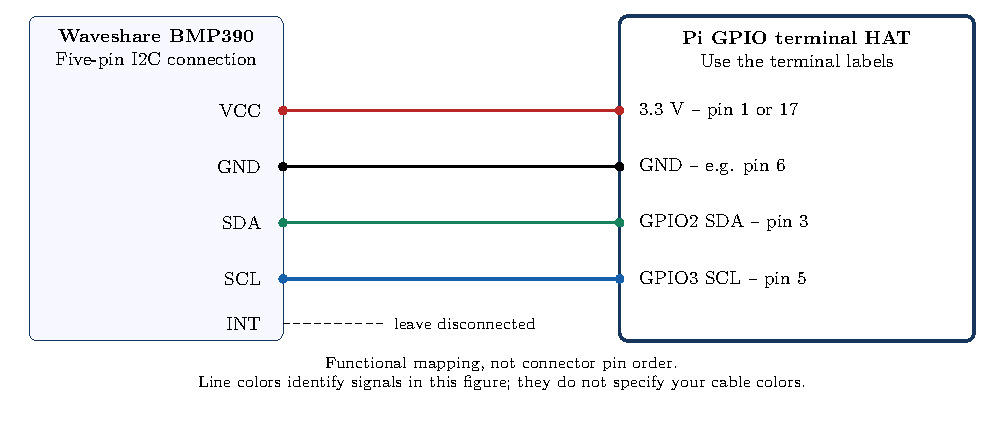
\includegraphics[width=\linewidth]{figures/BMP390 to GPIO terminal HAT.pdf}
\captionof{figure}{BMP390 to the GPIO terminal HAT: four connections; INT stays open. The diagram maps signal labels, not the physical order of the plug.}
\end{center}

\begin{enumerate}
\item Shut down the Pi and disconnect its power before changing connections.
\item Identify VCC, GND, SDA and SCL from the module labels. Connect the four paths in the table and figure; leave INT disconnected.
\item Keep the ADS1115 wiring in place. If the HAT terminals are occupied, branch SDA and SCL using the separate connectors shown on the next page.
\item Check for shorts and loose strands, then restore power. Do not put the sensor into water or cover its pressure opening.
\end{enumerate}
\clearpage\subsection*{Share the I2C bus and enable acquisition}
\begin{center}
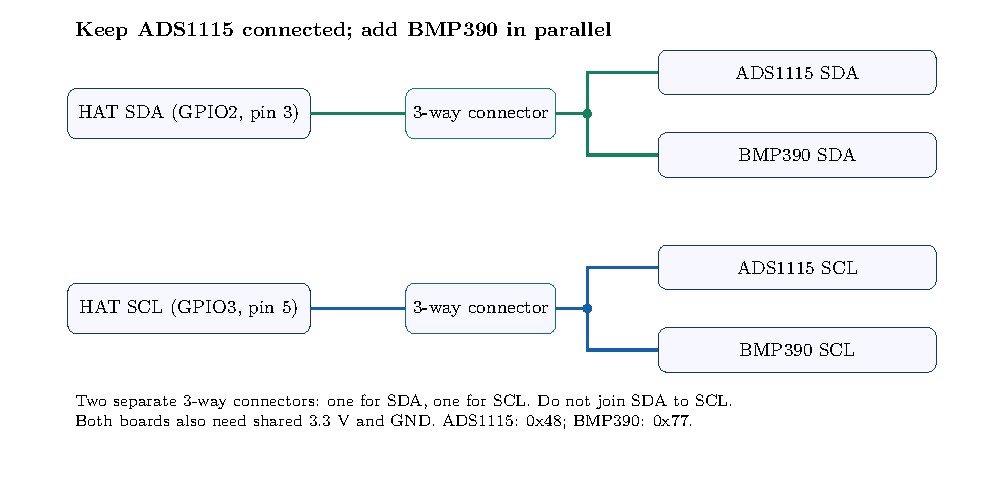
\includegraphics[width=0.94\linewidth]{figures/BMP390 and ADS1115 shared I2C.pdf}
\captionof{figure}{Two independent branches let ADS1115 and BMP390 share the bus without removing the moisture inputs. The power and ground connections from the first figure are also required.}
\end{center}
\textbf{Software channels.} Append these entries to the existing lab sensor array; preserve the other sensors and their calibrations. Bosch's official BMP3 driver handles factory compensation. Build with qmake (Qt 5) or qmake6 (Qt 6), then make. Back up the existing binary and configuration before restarting the user service.
\begin{lstlisting}
{"type":"bmp390_pressure", "id":"lab_barometer_pressure",
 "name":"Lab atmospheric pressure", "unit":"hPa",
 "intervalSeconds":60, "samplesPerReading":1,
 "params":{"device":"/dev/i2c-1", "address":"0x77"}},
{"type":"bmp390_temperature", "id":"lab_barometer_temperature",
 "name":"Lab barometer temperature", "unit":"degC",
 "intervalSeconds":60, "samplesPerReading":1,
 "params":{"device":"/dev/i2c-1", "address":"0x77"}}
\end{lstlisting}

Both channels share one physical driver. They use normal sensor health reporting and the durable cloud-upload queue under project \texttt{John-McCormack}. Adaptive idle polling may lengthen the 60-second recording interval. Failed readings are omitted; negative Celsius readings are supported.

\textbf{Expected result after starting acquisition.} The lab commissioning test produced about 1022.5 hPa and 21.7 $^\circ$C, with both channels healthy. These are example observations, not fixed calibration targets.

\textbf{Check operation.} Confirm I2C address \texttt{0x77} and chip-ID register \texttt{0x00 = 0x60}, then check fresh compensated pressure and temperature records and the two corresponding health components. An address response alone does not establish valid measurements. Large existing upload queues may delay cloud appearance.

Pressure is local absolute pressure in hPa, not sea-level corrected weather pressure or water pressure. Temperature is sensor temperature; Pi heat and enclosure heating may bias it above ambient air. Keep the module inside a dry, vented enclosure, away from the Pi's heat. Leave its pressure port open to air; do not seal, pot or immerse it.

\href{https://www.waveshare.com/wiki/BMP390_Barometric_Pressure_Sensor}{Waveshare wiring and module documentation}\quad
\href{https://github.com/boschsensortec/BMP3_SensorAPI}{Bosch compensation driver}
